\fancyhead[LO]{{\scriptsize {\FA \ }我们最幸福 {\FA } 妈妈的发明}}%奇數頁眉的左邊
\fancyhead[RO]{{\tiny{\textcolor{Gray}{\FA \ }}}\thepage}
\fancyhead[LE]{{\tiny{\textcolor{Gray}{\FA \ }}}\thepage}
\fancyhead[RE]{{\scriptsize {\FA \ }我们最幸福 {\FA }  妈妈的发明}}%偶數頁眉的右邊
\fancyfoot[LE,RO]{}
\fancyfoot[LO,CE]{}
\fancyfoot[CO,RE]{}
\chapter*{10 {\FA } 妈妈的发明}
\addcontentsline{toc}{chapter}{\hspace{5mm}10 \textbf{>}\ \ 妈妈的发明}
\vspace{5mm}
\begin{flushright}
	\textcolor{PinYinColor}{\EN \huge{Mothers\\
	of Invention\\
	\ \\}}
\end{flushright}
\begin{figure}[!htbp]
	\centering
	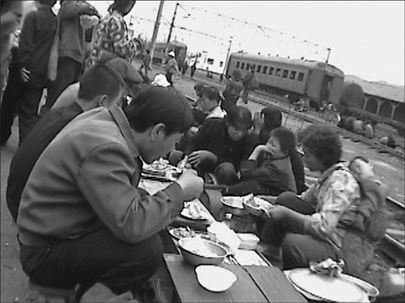
\includegraphics[width=6cm]{./Chapters/Images/10.jpg}
	\caption*{清津的一个临时餐饮摊点}
\end{figure}


宋女士没有参加儿子的葬礼。悲痛,饥饿和过去几年积累的压力彻底压垮了她的身心。她再也不忍心回到儿子死在里面的那个窝棚。“我留下他一个人孤零零的死去,是我留下了他。”她反反复复叨念着。她开始绝食。她在街上漫无目的的游荡,直到昏倒。\\

她的女儿们都外出去找她,最后发现她躺在在离家不远的荒草里,饿的已经神志不清,体温也很低。当时是3月下旬,但是夜间气温还是低的足以让一个营养不良的人毙命。当女儿们看见母亲的样子时,都被吓了一跳。宋女士曾经颇为得意自己那一头浓密卷曲的黑发;现在却披头乱发的肮脏不堪。衣服上也满是泥土。她们把她带回二女儿的家,脱下衣服,就像个孩子一样,给她好好的洗了一个澡。实际上,此时52岁的宋女士瘦的体重和玉熙8岁的儿子差不多。女儿们凑了点钱买了一袋面条给她。经过十五天适当饮食的调理,宋女士慢慢恢复了理智,想起发生了什么,然而这又一次让她对自己的不幸陷入绝望。\\

3年之内,走了三个至亲──婆婆死于1996年,丈夫死于1997年,儿子死于1998年。宋女士现在一无所有,包括伟大领袖,她对他的死与自己丈夫、儿子的死感到一样的悲痛。\\

她最后鼓起勇气回到了家,那个让她充满罪恶感的窝棚;她一个人对于家里去世的人负有责任。回去的路上,她边走边看看那个光秃秃的小山,只看见几个简单的木牌子标记着最近填的新坟;她的二女婿为也埋在那个小山上的自己的丈夫和儿子也做了个类似的标记。到了家,她发现门虚掩着。她记得,因为没有锁,离开的时候把门钉死了,很明显有人把它打开了。她推开门,先探个头张望了一下,确保里面没有人。窝棚空空荡荡的。没人。也没东西。煮饭的破铝锅,吃饭用的便宜金属碗,几双筷子,儿子死时裹的毯子,都不翼而飞了。窃贼甚至连金日成、金正日画像上的玻璃都没放过,只留下了画像。\\

宋女士又出门了,现在连关门都省了。她现在没什么可以丢的了,只有自己一条命,就算这个她也无所谓了。她也想不通为什么她还活着。她想就这么一直走下去,直到昏倒。她想倒下就死了算了。但是不知怎么的,始终死不了。于是她又开始找些事情做。\\

饥荒中奇怪的一点就是:当事情坏到了极点,几十万的人死去时,一种从未有的创业精神反而冒出来了。社会主义食物配给系统的崩溃却给私人经济以机会。人们不可能所有人都长途跋涉到山里去采野菜,野果,或者扒松树皮;人们要去买吃的,就必须有人卖。北朝鲜需要商人:鱼贩子、屠户、面包师傅,去填补公共体系垮台后的空白。\\

所有的这些都是严重违法的,金正日比他父亲制定了更严格的条框来针对私人经济。“在社会主义社会,即使是粮食问题也要按社会主义的方式解决。市场和摊贩都会导致人们产生唯利主义,“在1996年12月的一次演讲中他这样说道,这也是金正日为数不多的几次承认粮食危机的讲话之一。除了能在家种些蔬菜,粮食不能在市场上公开买卖。卖大米或者其它谷物是严格禁止的;北朝鲜将之视为非法及不道德,是在共产主义意识形态的核心上扎刀。任何私下的努力都被冠以“经济罪犯”,相应的惩罚包括流放到劳动营,如果涉及腐败,可能会被处以极刑。\\

然而,另一方面如果个人不为自己着想,那么死亡就是板上钉钉的事情。一个人一天至少需要500卡路里的热量维持生命;仅仅靠在吃在树林里所能找到的东西,一个人是很难活过3个月。死到临头给像宋女士这样不情愿成为资本主义者的人以新的勇气。\\

在上次大米生意的血本无归之后,宋女士意识到,她要坚持一门最简单的生意,不要出差,不要很多启动资金。她最拿手的、也是唯一的畅销的技能就是厨艺。但是做饭变得越来越难,因为柴火越来越难找。附近的山都秃了,有树的地方人都到不了。\\

深思熟虑之后,宋女士决定把她未来的重心放在烤饼干上面。饼干只需要在烤炉里烤10分钟就好了,一捆柴火可以烤四到五批。它们比面包容易烤熟,而且饼干是快餐食品很适合那些赶路的人。\\

宋女士加入了她的小女儿容熙的饼干生意,时年容熙刚刚离婚──她的婚姻,在容熙发现丈夫是个无可救药的赌徒之后,三个月就宣告结束了。容熙借了些钱,买了些废铁,让钢铁厂里失业的电焊工给加工成烤炉。烤炉大致上是方形,分成上下两部分,在底下一层烧煤,而上面一层用来烤饼干。她还做了个饼干架子。宋女士和容熙还来回穿梭于城里的各个市场,从其它卖饼干的小贩那里取经。当时很多妇女都在卖饼干,有段时间,宋女士还去给她们帮工,边看边学。她也从其它小贩那里买些样品尝尝,对比一下。找到她们喜欢的口味,然后试图复制其配方。\\

她们的第一次尝试不尽如人意。第一批产品还不适合拿到市场去销售,即使是以北朝鲜的标准来看也是。为了不浪费宝贵的饼干原料,宋女士和女儿把失败的产品都吃了。最后,她们发现要多放些糖和酵母。而且她在配方里还加入牛奶。然后把生面团切成不同的形状,这样看上去真的很像是小甜饼──一种不是太甜且很容易消化的小零食。\\

宋女士每天早上5点起床做饼干。市场竞争的很激烈,她的饼干必须保持新鲜。她没有手推车甚至连用来卖货的木箱子也没有,只好把饼干放在塑料盆里,然后在用一个带子把盆子像背小孩一样背在背上,到行人聚集的主干道去卖,那里的竞争者会少些。她徘徊于市场里和火车站前面的大广场上。由于背还没好,当疼的时候,她就会双腿交叉盘腿坐在地上,把饼干盆放在膝盖上。\\

由于在事故中受伤的背还没有完全好,所以她就对着来往的行人吆喝兜售,一如过去她负责人民班时,需要吆喝大家收集可循环利用的废品及给祖国收集粪便一样。喊声充满热情。\\

“Gwajasassayo。”这些话以朝鲜语一种单调的语调唱着。意思是“买饼干喽。”\\

宋女士天生就是做生意的料。人们都被她的热情感染着;如果有人想买饼干,他们就会到她那儿去买,虽然可能有多过数打的人在卖饼干。一天14个小时下来,她口袋里大概会有100朝元──都是些5毛钱的钞票,可能还会有几袋其它的东西,有时是红辣椒,有时是几袋煤球,都是用来和她换饼干的。赚的钱刚刚够她买自己的晚餐和下一批烤饼的原料而已。拖走两条沉重的腿回到家后,往往精疲力尽,倒头就睡了,但是仅仅几个小时之后又要起来,一切都又要重复一遍。不同的是,她现在不再饿着肚子上床而已。\\

数以千计的妇女做着同宋女士一样的事情。他们都是个体户。他们没有固定的工作场所或者店面;他们不敢设立售货亭之类苏联改革时期街头上司空见惯的那种摊档。关于商业,除了被灌输的,所有的私有经济都是唯利是图的之外,他们没什么概念。但是饥饿和绝望,使得他们重新审视自由市场经济的概念,而这个概念又是当局宣传中所要求的永不涉及的禁区。在实践中,人们已经发展出一种在易物交易中衡量物品价值的技能;体力好的年轻人,可以到深山中砍到柴火,而宋女士到不了那么远,就只能用她的饼干来交换柴火。如果你有梯子,你就可以从电线杆上收集到铜线\footnote{没有什么危险,因为没有电。}然后用于换吃的。如果你有那些废弃工厂的钥匙,你就可以拆掉那些机器、窗户和地板以作他用。\\

不论是烤盘还是小推车,都是个人手工制作的,工厂早就关门了。女人们把帆布剪成小块,把捡来废弃的橡胶融化,制成简陋的运动鞋。旧轮胎、木门、铁丝被用于制作那种往返于市场和家里的装货用的小推车。\\

人们什么都是自学。一个没接受过什么教育的矿工,找到一本关于东方医药的书,潜心研读后,瞭解了清津附近山上所能采到的草药及其功效。他成为和医生一样好的草药专家,而且由于身体好,他能到更偏僻的地区采到草药。\\

医生,也不例外,有他们的赚钱之道。他们自己没有药,但是他们可以在医院或者在家进行简单的诊疗。油水最丰的就是堕胎,严格来讲在北朝鲜没有特别许可,堕胎是非法的,尽管如此,堕胎却是控制生育的一种通常做法。虽然饥饿降低了人们的性欲和繁殖力,但是仍然有妇女怀孕,家里不想要这些孩子,因为他们养不起孩子。几年前,当玉熙带一个朋友去堕胎时,那时候花费大概是400朝元,差不多相当于8公斤大米的价格,但是近来价格低到甚至提一桶煤去就可以了。\\

金医生没有受过做手术的训练。她靠她的笔生存,写医嘱说病人需要离岗休病假。旷工在北朝鲜可是要在拘留所被拘留30天,即便是工作单位再也发不出工资。但是人们需要时间外出去找吃的和燃料。作为回报,他们会给金医生一些他们所能找到的任何吃的东西作为礼物。她厌恶写假的医嘱──这违背了她入行时,对这个职业,对祖国的所有信约。\\

美兰足智多谋的母亲又开始了另外一门困难时期非常红火的生意。通过大女儿的关系,她弄到开磨坊的许可。不像她的冰激凌和豆腐生意,没有电就做不成,磨坊用的是传统工艺,完全是人工运作。在煤矿为巷道做支撑的泰宇为磨坊做了一个木头的棚子。当安装棚顶的时候,邻居们都来帮忙,甚至恰好在家休假的俊相都来帮忙了。磨坊刚刚建成,四邻八乡的邻里们就带着玉米来磨坊了。对他们来说,直接买玉米要便宜的多,而且可以视需要决定将多少玉米磨成玉米面,包不包括玉米秆子、叶子、玉米芯子、玉米壳──甚至你可以决定要不要混些锯末进去。而且只有磨成很细很细的粉末,这样的混合物才能被消化,所以磨坊是一门很重要的营生。\\

如果你没什么可以卖的,你就卖了自己吧。\\

虽然金日成早就取缔了妓生园\footnote{妓生园是朝鲜的妓院。──译者},卖淫却从来没有被消灭,只是在非常小心谨慎之下,由个人安排在普通人的住所里悄悄进行。饥荒不仅逼的妓女们走向大街,还产生了新的妓女类型──通常是已婚的年轻妇女,从事卖淫仅仅是为了给孩子买吃的。她们通常只要一袋面条或者几个红薯作为嫖资即可。她们一般聚集在清津主火车站外的广场上。在广场上,总有几百人长时间的等着火车,靠着这些人在广场上来回徘徊的掩护,她们也就变得无影无踪。找生意的女人们好像参加鸡尾酒会一样,来回穿梭于人群之中。她们的着装很邋遢低调,如果她们穿太短的裙子,太短太紧身的衬衣或者蓝色牛仔裤,或者佩戴首饰的话,马上就会被公众标准警察逮捕,所以妓女们就采用涂抹浓重的红色口红作为标记,并且用眼神挑逗过往的男人。\\

玉熙住在丈夫所工作火车站的正对面。每当她看见这样的女人时,她总会很尴尬的低下头,尽量避免目光对视。然而有一个女人,却总是想方设法的同她进行目光交流,有时候还会对玉熙笑笑。她比其它人穿的要好一点,更自信,甚至可以说很职业。\\

有一天,当离一出门的时候,玉熙发现那个女人就在她家门口几米之外的地方,看上去好像在等她。\\

“听着,姐姐。”她很亲热的说着。“我兄弟刚刚到这里,我们有些事情想私下聊聊,你能借个房间给我们吗?”\\

此时,她朝在她后面来回踱步的一个男人点点头,他侧着脸。玉熙原来对这种皮肉生意感到有点恶心,但是当真的遇到时,她却意识到这是个不错的赚钱机会。她丈夫外出工作,孩子在学校上课。那个妓女用她一个房间一个小时付了50朝元。后来她就经常会来,除了付租房的钱,有时候甚至还会给玉熙的孩子一些糖果。\\

当然,这是非法的,但是回过头来说,现在也是司空见惯了。提供服务收取酬劳都是犯法──不管是卖淫还是修自行车。但是现在谁又在乎呢?为了生存,每个人都在铤而走险。\\

大多数的商品交易都在老的农贸市场上进行。即使在共产主义的黄金时期,金日成也不得不默许某些市场的存在,但这只限于人们出售自己菜园里种植的副食品。当孩子还小的时候,宋女士手头上如果有些余钱的话,就会常常去位于她公寓附近空地上的市场,买些鸡蛋,给孩子们当早餐补补营养。根据季节的不同,她还会买些在太阳下晒成的红辣椒干,咸鱼或者大白菜。人们还可以在市场买到二手的衣服,鞋子,和碗碟,在市场上交易全新的商品是被严格禁止的,那些东西只能在国营商店里买卖。\\

在90年代,即使是在饥荒非常严重的清津,人们时时刻刻都被死神危险着,然而令人不解的是,市场上却出现了越来越多的食品。大白菜、萝卜、生菜、西红柿、洋葱和马铃薯都能在市场上买到。这些蔬菜都是来自分布于山村里的一些秘密菜园。对于农民来说,他们发现最好的生存之道就是在坡地上开荒,即使是在过去认为坡度太陡不适宜耕种的地方。所有的精力都被倾注到这些自留地里,一排排的蔬菜如同打字机的键盘整整齐齐的,豌豆和南瓜的蔓藤都爬上搭好的棚架,而集体农庄的作物就被随意的打理一下。\\

市场上也突然有了白米、大量的白米,40公斤装在粗麻布袋子里,外面印着罗马字母\footnote{罗马字母指UN联合国,WFO世界粮食计划署,EU欧盟。}还有联合国相互交叉的橄榄枝的标志,有些还有美国国旗,每个北朝鲜人都从宣传栏上认识了这些标志,不同的是,宣传栏上出现这些标志的时候通常都滴着血或者被刺刀刺穿。\\

为什么米袋子上会出现北朝鲜死敌的旗帜?有人告诉宋女士这是北朝鲜军队从美国战争贩子那里俘获的战利品。有一天,宋女士看见一队卡车驶离港口,车上装着的都是这样的粗麻布袋子。虽然卡车都挂着民用车牌,但是宋女士清楚它们都是军用卡车──因为没有其它人会有汽油──她后来估摸着这是人道主义救援,军队有人把这些物资拿到市场上牟利。\\

不管它来自那里,清津人看到这些大米都非常高兴,大米在公共配给系统中已经消失很多年了。\\

每次去市场,宋女士总会见到很多让她吃惊的东西。桃子、葡萄、香蕉。她已经记不得上一次见到香蕉是什么时候的事情了──也许是20年前,长博买了些给孩子吃。有一天,她还看到橙子,真正的橙子!宋女士从来没尝过橙子──她只从图片上看到过。还有一天,她看见一种带着斑点的黄棕色水果,顶上还带有绿色的刺。\\

“这是什么东西?”她问一个朋友,那个朋友告诉她那是菠萝。\\

还是第一次,市场的家庭日用品是如此廉价,即使是北朝鲜人也买得起了。邓小平开始于70和80年代经济改革的成果也渗透进了北朝鲜。市场上充斥着从中国来的信纸、钢笔和铅笔、沐浴露、洗发水、指甲钳、剃须刀、电池、打火机、雨伞、玩具车、袜子。长久以来,北朝鲜坚持什么都要自产,使得这些稀松平常的东西都变得珍贵无比。\\

着装也能说明一些问题,外面世界的色彩也慢慢侵入了。粉红、黄、橘红、青绿──衣服的色彩也同市场上的热带水果一样多姿多彩了,面料也比北朝鲜自制的更柔软,更闪亮。偶尔,在市场上你还能见到去掉了商标,质量更好的衣服。商贩偷偷的说这些衣服是来自Arehdongae,意思是“南边的村子。”意指南韩。人们都愿意付更多的钱去买产自敌国的衣服。\\

每次宋女士去市场,都觉得它变得一天比一天大。现在那里不再是老年妇女蹲在泥地上铺着防水布的那个市场了;现在是数百计商贩的箱式或手推车式摊位的市场。商贩们买来桌子、柜台和大阳伞以免他们的商品被太阳直射。\\

清津最大的市场发起于水南(Sunam)河附近的工业废弃地,从那里经港口很快就可以到市中心。在荒凉的化纤厂旧址后面,水南市场最后成为北朝鲜最大的市场。它的形式同亚洲其它地方的市场没什么区别──几条走道是卖食品的,其它的有卖五金、锅碗瓢盆、化妆品、鞋类、服装。直到2002年,金正日才勉强将市场合法化。然而清津当局早几年就非正式的认可了市场的存在,并加以管理。市场管理部门对入场的摊贩每天收取70朝元的租金──相当于1公斤大米的价格。付不起租金的摊贩就在市场大门处支起摊位,所以市场延伸的更远,一直快到河堤边的陡坡。宋女士的饼干生意从不曾到可以单独租用摊位的程度。她也不想付租金。但是她确实成为小贩组织的一员,在松片(Songpyeon)市场的边缘做生意,这个市场位于港口的西侧,在那里一旦赚到一点钱,她就要换个地方。\\

市场像个磁铁,吸引着各式各样的营生。在水南市场外,沿着歪歪扭扭的一排蜀葵后是一条刷着白灰的墙,前面排着一排木制推车。他们的主人通常就在车上睡觉,等着需要拉货的雇主。清津没有出租车,甚至连中国那种人力车、三轮车都没有\footnote{朝鲜当局认为那些东西有失体面。}。但是人们不得不把自己作为搬运工填补这个空缺。理发师是由政府的便利局训练出来的,而这个机构应该提供人们需要的各项服务,此时也在市场设立了流动的理发服务点。他们要的只是一把剪子,一块镜子就可以开张了。他们一般在靠近食品市场的地方工作,因此也常常以为剪下来的碎头发飘到吃的上面而同其它商贩吵架。理发师要动作很快,一只眼睛要确保剪刀不把耳朵剪破,另外一只眼睛要小心警察,如果被抓住从事私人生意,他们所有的工具都会被没收。即便如此,这还是有利可图的。因为即便饥肠辘辘,妇女们仍会用最后一块钱去烫发。\\

在沿着铁道的市场上,人们用砖块支起一块木板,小桶反过来当凳子,设立了移动的饮食摊点。顾客也吃的很快,他们用勺子快速的扒着小金属碗里盛的汤或者面条。用来加热食物的圆柱状金属炉子不会比油漆桶大,采用传统的方式,摇扇子生火。女人们背上背着孩子、蹲着生火的情景也不少见。\\

商贩绝大部分都是妇女。按朝鲜人的传统,商人的地位很低,所以一般也就是女人去做。即便在90年代,市场有很大发展后仍然如此。男人们要待在工作单位,而工作单位是北朝鲜人生活的中心,一切都要围绕着它,但是妇女有大把的闲暇时光,她们可以找借口逃脱自己的本职工作。从清津逃出来的脱北者朱成夏,现在在首尔当了一名记者,他告诉我,他相信金正日为了减缓饥荒带来的压力,不得不默许妇女从事私人经济活动。“如果不准阿玛们\footnote{朝鲜已婚妇女。}去工作,可能会激起民变。”他说。\\

结果就是,新经济体内,女人的作用越来越重要。男人受困于拿不到工资的工作单位;妇女们则在赚钱。“男人还不如一条看家狗有用。”有些阿玛们私下这样抱怨。虽然女人们更高的收入改变不了千百年来形成的家长制文化,但是她们也确实得到一定程度的独立。\\

从外表看来,清津并没有什么变化。空空荡荡的柏油路傍,树立着一样的,灰色外墙的斯大林式样的办公楼。路边仍然点缀着褪了色的,颂扬金正日和劳动党的红色宣传栏。确实,这里的时间仿佛停止了,仿佛时间还停留在70年代的世界。但宋女士很清楚。她生活在一个浑沌的糟糕世界里。这里黑白颠倒、好坏不分。妇女比男人有钱。市场上满是食物,数量之多,是大多数北朝鲜人一辈子没有见到过的,但是另一方面,人们仍然大量饿死。劳动党员也被饿死;而那些从不在乎祖国的人却大把的赚着钱。\\

“Donbulra。”宋女士低声的咒骂着。金钱的奴隶。\\

在过去,她觉得很心安理得,多多少少大家都一样的穷。现在,她看见富者愈富;而穷者愈穷。早10年,穿皮鞋、穿新衣服的人会被视为经济罪犯。有些人即使努力工作仍然改变不了挨饿的境地。通货膨胀失去控制。在黑市,大米的价格在1998年底飙升到两百朝元1公斤。即使工资恢复了,一个普通的办公室人员或者一个教师的月工资,还买不起一家人2-3天所需的食物。孩子们跪在地上四处搜寻,捡拾那些从麻布袋里散落在地上的米粒或者玉米粒。\\

她认识一个男孩,成哲,9岁。他常常和父亲一起来市场,他父亲很粗鲁,因为卖梨子,其它商贩都叫他“梨子大叔”。但是梨子生意不好,梨子大叔很难靠此养活全家。\\

“你为什么不像其它男孩一样,去弄点吃的?”梨子大叔有一天在市场上这样告诉他的儿子。\\

成哲是个很听话的孩子。他走到一个男人们喝酒吃蟹的摊挡傍边。就在他父亲摊点的侧面,突然他喊肚子疼。他吃了些丢在地上的一些煮过的鱼内脏。在梨子大叔能用仅有的一点钱送他去医院看医生之前,他就死于急性食物中毒。\\

几乎没有一天,宋女士不是在死亡在线挣扎。虽然自己与自己家庭经历了这么多,她还是不能习惯于这种持续不断的死亡。有一天,从市场回家的路上,她绕道去了下火车站,希望能卖掉剩下的饼干。工人们正在清扫站前广场。许多人拉着一架沉重的木拖车走过。宋女士好奇的想看了看他们拖得什么东西。里面堆满了尸体,差不多有六具,都是前一天晚上火车站死掉的人。一些瘦骨嶙峋的肢体伸在车外,一个头颅垂了下来,在地上拖着。宋女士睁大了眼睛;那是个40来岁男人的头颅。他的眼睛依稀还在眨巴着,还没完全死去,但是也差不多可以用车拖走了。\\

宋女士禁不住的想起自己死去的亲爱的丈夫和儿子。他们能死在自己的家里、自己的床上,而且她还能给他们体面的葬礼,想到这点她感到欣慰无比。\\
